\section{Versuchsziel}
Die Bestimmung der Austrittsarbeit der Elektronen für das Metall Wolfram
unter Verwendung des glühelektrischen Effekts. Zudem soll die Kennlinie einer
Hochvakuumdiode bestimmt werden, in welcher der glühelektrische Effekt untersucht
werden kann.
\section{Theorie}
\label{sec:Theorie}
\paragraph{Potentialtopf}

Ein Elektron im Atomgitter des Metalls befindet sich, in grober Nährung,
in einem konstanten einheitlichen Potential. Das Potential außerhalb des Metalls
ist um den Faktor $ \Phi$ größer, dieses Potentialtopfmodell ist in der Abbildung
\ref{fig:Pot} dargestellt. Um das Metall verlassen zukönnen muss ein
Elektron die Austrittsarbeit $\symup{e}_0 \cdot \xi$ leisten.
\begin{figure}
  \centering
  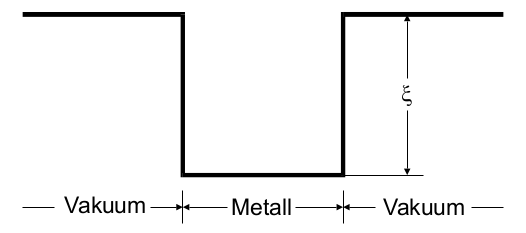
\includegraphics[height=3cm]{logos/Potentialtopf.png}
  \caption{Potentialtopf eines Metalles \cite{Anleitung}.}
  \label{fig:Pot}
\end{figure}
\FloatBarrier.
\paragraph{Fermi-Dirac Verteilung}
Die Fermi-Dirac Verteilung gibt die Wahrscheinlickeit an für die ein möglicher
Zustand mit der Energie $E$ im thermischen Gleichgewicht besetzt ist. Die
Fermi-Dirac-Funktion ist gegeben durch
\begin{equation}
  f\left(E\right) = \frac{1}{\exp\left(\frac{E - \zeta }{\symup{k_B}T+1}\right)}
\end{equation}
gegeben, dabei bezeichnet $T$ die Temperatur, $k_B$ die Boltzmann-Konstante und
$\zeta$ die Fermische Grenzenergie. Die Funktion ist in der Abbildung \ref{fig:FD}
dargestellt. Um aus der Metalloberfläche auszutretten müssen die Elektronen eine
Energie von $\zeta + e_0 \cdot \Phi$ besitze, da diese Energiewerte auch im
Schmelzpunkt von Wolfram noch groß im vergleich zu $k_B T $ sind kann die Närung
\begin{equation}
  f\left(E\right)= \exp\left(\frac{\zeta - E}{k_B T} \right)
\end{equation}
benutzt werden.
\begin{figure}
  \centering
  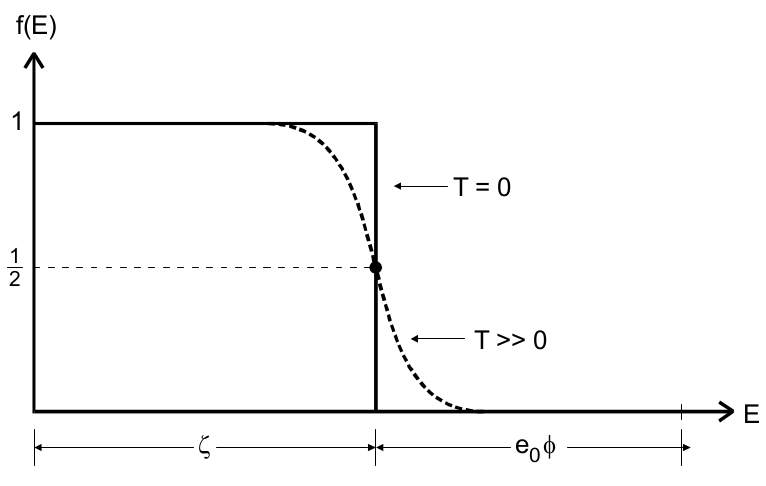
\includegraphics[height=5cm]{logos/Fermi-Dirac.png}
  \caption{Fermi-Dirac Verteilung am absoluten Nullpunkt
  \texorpdfstring{$T = 0$}{math} und \texorpdfstring{$T >> 0$}{math}
  \cite{Anleitung}.}
  \label{fig:FD}
\end{figure}
\FloatBarrier
\begin{equation}
  j_S(T) = 4\pi \frac{e_0 m_0 k_B ^2 }{h^3} T^2 \exp \left( \frac{-e_0 \Phi}{k_B T}\right)
\end{equation}

\begin{figure}
  \centering
  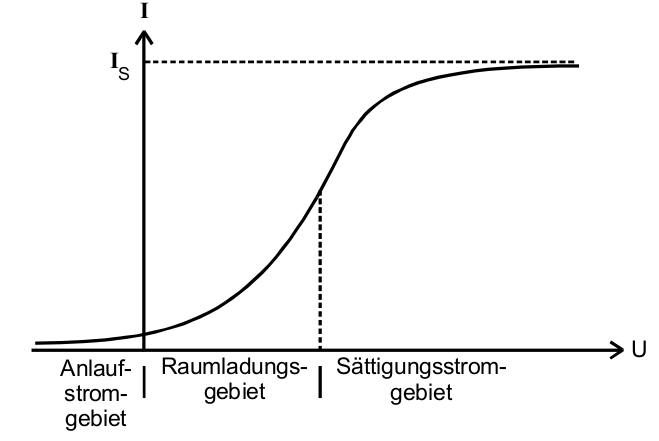
\includegraphics[height=5cm]{logos/Kennlinie.png}
  \caption{Kennlinie einer Hochvakkumdiode \cite{Anleitung}.}
  \label{fig:KL}
\end{figure}
